\section{Marco conceptual redes complejas}

\subsection{Glosario}
\begin{itemize}
    \item \textbf{Diámetro de una red}: Es el número de aristas de la distancia geodésica más larga
    entre un par de vértices de una red.
    \item \textbf{Distancia geodésica:} Es el camino más corto entre un vértice y otro a través de una red. Es posible exista más de una camino geodésico.
    \item \textbf{Distribución de grado} Es el recuento del número de vértices en un grafo que tienen un grado dado, tomando el número de vértices que tienen un grado dado este puede seguir una distribución de probabilidad.
    \item \textbf{Grado de un vértice}: Es el número de conexiones asociadas a un vértice en un grafo.
    \item \textbf{Grafo}: Un grafo es un conjunto de vértices conectados con aristas
    \item \textbf{Hub}: Vértice en una red libre de escala que tiene un mayor grado con respecto al resto.
    \item \textbf{Sistema complejo:} Un sistema complejo es aquel que esta compuesto de muchos componentes que interactúan.,Se encuentran propiedades emergentes que no se pueden explicar sólo tomando en cuenta a sus componentes individuales, en otras palabras el todo no es la simple suma de sus partes.
    \item \textbf{Sistema complicado:} Es un sistema el cual puede ser descrito completamente a partir de sus componentes, no presenta comportamiento emergentes.
\end{itemize}


\subsection{Redes complejas}

Una red o grafo\cite{Newman2003}
es un conjunto de elementos, vértices o nodos los cuales están conectados por aristas. Los sistemas reales pueden ser modelados como redes. Algunas redes reales son la Internet, redes sociales de conocidos, redes de estructura en organizaciones, redes de intercambio de bienes, redes neuronales ,redes metabólicas, redes de citaciones y muchas otras.

El estudio de redes, puede realizar usando la teoría de grafos. Los estudios típicos en redes se aplican en áreas como la sociología donde se pueden modelar redes a partir de los resultados de cuestionarios acerca de las relaciones interpersonales como es el caso de la figura \ref{fig:contactosSexuales}, en estos modelos sociales se pueden encontrar resultados interesantes como es el caso de la

\begin{figure}[H]
    \centering
    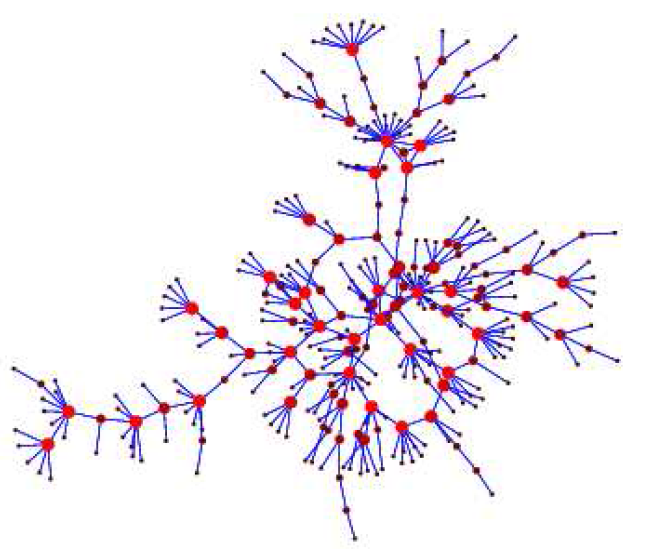
\includegraphics[scale=0.3]{Capitulo2EstadoDelArte/imagenes/contactos.png}
    \caption{Ejemplo de red de contactos sexuales \cite{Newman2003}}
    \label{fig:contactosSexuales}
\end{figure}

\subsubsection{Definición formal}

Una red o grafo se puede definir así:

\begin{equation}
    G = (V,E)
\end{equation}

Donde $V$ es el conjunto de nodos y $E$ es el conjunto de aristas. Una arista es un par de vértices $(i,j)\in V^2$, en el caso de los grafos dirigidos este par es ordenado. Los enlaces también pueden tener un paso asociado, el cual es un valor numérico. Las redes tienen las siguientes propiedades básicas:

\begin{enumerate}
    \item Dos vértices distintos son adyacentes si y sólo si hay una arista que los conecta
    \item Una arista es incidente a un vértice, si este hace parte de ella
    \item El vecindario de un vértice son todos aquellos que se conectan directamente a través de una arista
\end{enumerate}

\subsubsection{Propiedades de redes complejas}

Las propiedades de una red compleja son\cite{barabasi2002linked}:

\begin{itemize}
    \item Distribución de grado: es la probabilidad que un nodo tenga un número determinado de conexiones
    \item Coeficiente de agrupación: es la probabilidad que tomando un número determinado de nodos se obtenga un grafo completo, el cual consiste en que todos lo nodos se conectan entre sí.
    \item Longitud promedio de la red: Es el promedio de todas las distancias minimas entre los vértices
\end{itemize}

\subsubsection{Clasificación de las redes complejas}

Las redes se clasifican de acuerdo a sus propiedades estructurales en

\begin{enumerate}
    \item Redes aleatorias, las cuales tienen una distribución de grado Poisson
    \item Redes libres de escala: las cuales tienen una distribución de grado de ley de potencia.
    \item Redes de mundo pequeño: son aquellas redes cuyo coeficiente de agrupamiento es levado y la distancia promedio entre los vértices es un valor proporcional al logaritmo del número de nodos.
\end{enumerate}

\subsubsection{Modelos de generación de redes complejas}

Actualmente existen muchos modelos en la literatura, los más relevantes son:

\begin{enumerate}
    \item Modelo de Erdos-Renyi\cite{Erdos1959}: es utilizado para generar redes aleatorias. El método consiste en conectar los nodos entre sí con igual probabilidad. La distribución de grado que se genera en estas redes es Poisson.
    \item Modelo de Albert-Barabasi\cite{Barabaacutesi1999}: permite generar redes libres de escala, mediante un mecanismo de enlace preferencial, en el cual los nodos que tienen mayor grado son los que tienen mayor probabilidad de recibir nuevas conexiones, generando así una distribución de grado de ley de potencia.
    \item Modelo Watts y Strogat\cite{Watts1998}: el cual genera redes libres de escala mediante un mecanismo de colocar y quitar enlaces, de tal forma la distancia promedio entre cada par de nodos sea la menor posible.
\end{enumerate}

\newpage
